\documentclass[a4]{article}

\usepackage[T1]{fontenc}
\usepackage[utf8]{inputenc}

\usepackage{amsmath}
\usepackage{amssymb}
\usepackage{a4}

%opening
\title{
%%Tentative titles :
%Looking where it is worth looking
%Learning where to see
Learning where to look for a target before seeing it
%Where is My MNIST?
}
\author{}

\begin{document}

\maketitle

\begin{abstract}
A realistic system for object categorization should be able to find the target in possibly large images, independently of its position in visual space. Current solutions leverage this solution by processing the different hypothesis (classes) at all possible spatial configuration. However, this can be costly in terms of computing time especially without dedicated parallel hardware. %
We explore here a solution inspired by the anatomy of the human visual system, that is, the combination of a foveated sensor with the capacity of rapidly moving the center of fixation using saccades. Indeed, the position and category of objects in images are a priori independent and we hypothesize that the retinotopic map overlays a central area dedicated to object categorization and a peripheral area dedicated to
Using this hypothesis, we formalize this problem in a probabilistic setting which allows us to build two parallel but interactively connected system: a classical image classification algorithm assuming that gaze is centered on the object on one side and a system learning to infer the position of the target on the other. Until the classification is confident, the system performs a saccade to the most likely position in the image. Overall, the computational cost of this strategy is less than that in holistic methods. %
We tested this framework on a simple task of finding digits in a large, cluttered image. Results demonstrate that it is possible to correctly learn the position of a target from a given class, and this before actually seeing a foveated image of the target. We compare the results of this model with classical psychophysical results in visual search. This provides evidence of the importance of such strategies in computer vision and we highlight some predictions of our model.
\end{abstract}

\newpage
% !TEX root = paper.tex
% !TEX encoding = UTF-8 Unicode
% -*- coding: UTF-8; -*-
% vim: set fenc=utf-8
% !TEX spellcheck = en-US
\section{Introduction}
\label{sec:intro}
\paragraph{Problem statement.}
%------------------------------%
%: see Figure~\ref{fig:intro}
\begin{figure}[b!]%%[p!]
	\centering{	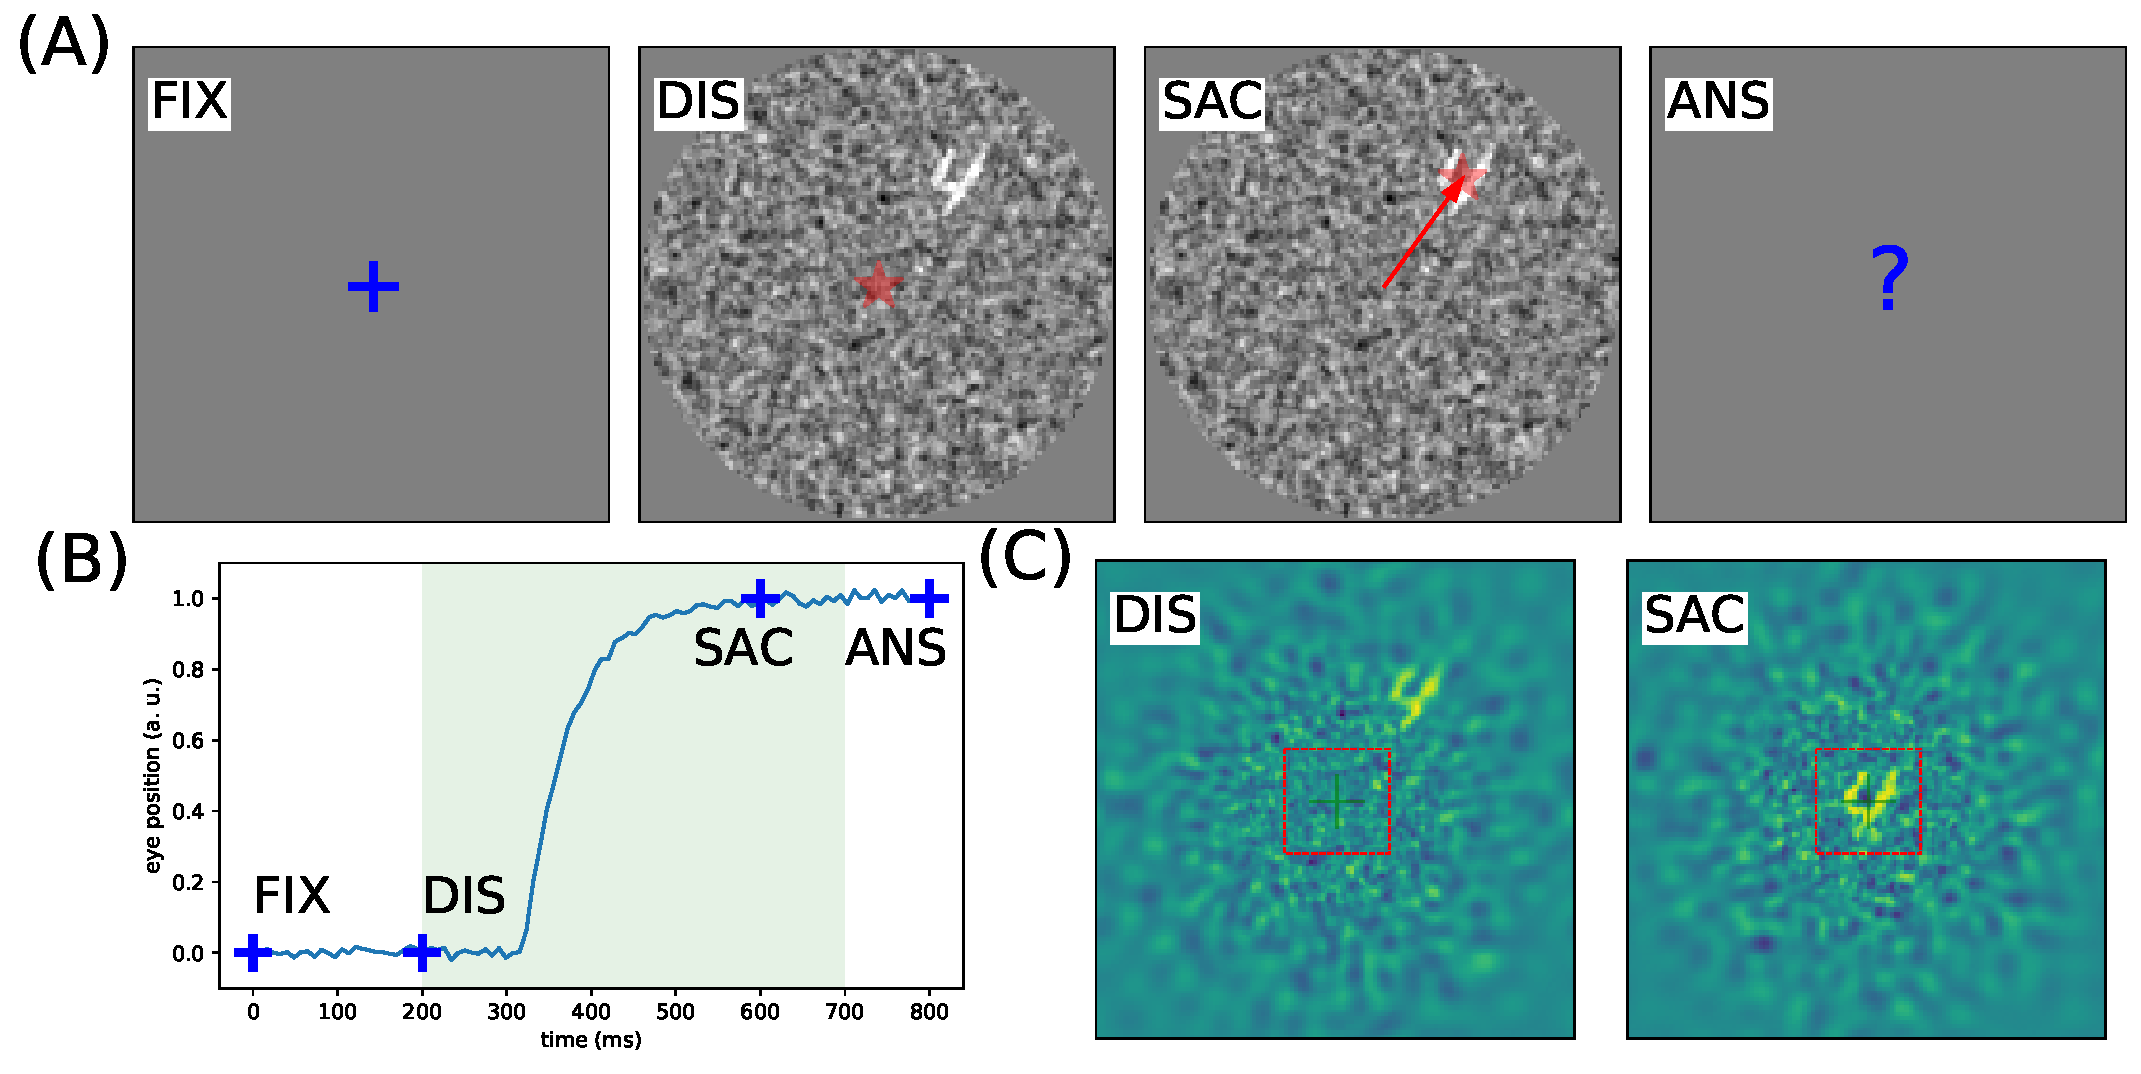
\includegraphics[width=\linewidth]{fig_intro}} %
	\caption{%
		{\bf Problem setting}: In generic, ecological settings, the visual system faces a tricky problem when searching for one target (from a class of targets) in a cluttered environment. It is synthesized in the following experiment: %
		\A After a fixation period \FIX\ of $200~\ms$, an observer is presented with a luminous display \DIS\ showing a single target from a known class (here digits) and at a random position. The display is presented for a short period of $500~\ms$ (light shaded area in B), that is enough to perform at most one saccade (here, successful) on the potential target \SAC . Finally, the observer has to identify the digit by a keypress \ANS . %
		\B Prototypical trace of a saccadic eye movement to the target position. In particular, we show the fixation window \FIX\ and the window during which a saccade is possible (green shaded area). %
		\C Simulated reconstruction of the visual information from the (interoceptive) retinotopic map at the onset of the display \DIS\ and after a saccade \SAC , the dashed red box indicates the visual area of the ``what'' pathway. In contrast to an exteroceptive representation (see A), this demonstrates that the position of the target has to be inferred from a degraded (sampled) image. In particular, the configuration of the display is such that by adding clutter and reducing the size of the digit, it may become necessary to perform a saccade to be able to identify the digit. The ``where'' pathway mediating the action has to infer the location of the target \emph{before seeing it}, that is before being able to actually be able to identify the target's category using the ``what'' pathway. %
		\label{fig:intro}}%
\end{figure}%
%%------------------------------%
The promise of artificial vision to identify objects in natural images is ever increasing. Image processing algorithms recently outreached the performance of human observers in specific image categorization tasks~\citep{He15}. Initially trained on energy greedy, high performance computers, they are now designed to work on more common hardware such as desktop computers with a decent GPU~\citep{Sandler18}. However, these algorithms are still outperformed by humans for simple tasks. Take for instance the case of an encounter with a friend in a crowded café. To catch the moment at which he will arrive, you need to visually search for his face despite all the remaining sensory clutter. To do so, you need to scan relevant parts of the visual scene with your gaze. Doing a saccade at these locations, you will be able to recognize your friend. The main difficulty of this task is to learn to categorize this particular object class given all possible spatial configurations and respective geometrical visual transformations. Such a visual experience can be formalized and simplified in a way reminiscent to classical psychophysical experiments: An observer is asked to classify digits (for instance as taken from the MNIST database) as they are shown on a computer display. However, these digits can be placed at random positions on the display, and visual clutter is added as a background to the image (see Figure~\ref{fig:intro}-A). This opens the possibility that the position of the object may be detected in the clutter without being identified in the first place  (see Figure~\ref{fig:intro}-C). This defines more precisely our problem: how can we localize an object in a large image while knowing \emph{a priori} its category but not its identity? This generic visual search problem is of broad interest in machine learning, computer vision and robotics, but also in neuroscience, as it speaks to the mechanisms underlying foveation and more generally to low-level attention mechanisms.

Inherent to this problem is the combinatorial explosion implied by an increasing number of parameters. State-of-the art classification architectures consequently contain many millions parameters while still handling relatively small images, with subsequent energy consumption increase. This introduces a trade-off between efficiency (fast enough to detect visual objects in a glance in autonomous driving as well as being able to extend it to resource-constrained devices like mobile phones) and average accuracy. Globally, this performance is  still lower than that of humans. Indeed, the human visual system can perform such a feat both rapidly, --~in less than 100 ms~\citep{Kirchner06}~-- and at a low energy cost ($<5~W$). On top of that, it is mostly self-organized, robust to visual transforms or lighting conditions and can learn with a few examples. If many different anatomical features may explain this efficiency, a main difference lies in the fact that its sensor (the retina) combines a non homogeneous sampling of the world with the capacity to rapidly change its center of fixation. Indeed, on the one hand, the retina is composed of two separate systems: a central, high definition fovea (a disk of about 6 degrees of diameter in visual angle around the center of gaze) and a large, lower definition peripheral area. On the other hand, the retina is attached on the back of the eye which is capable of low latency, high speed eye movements.  In particular, saccades allow for efficient changes of the position of the center of gaze: they take about $200~\ms$ to initiate, last about $200~\ms$ and usually reach a maximum velocity of approx 600 degrees per second. This behavior is prevalent during our lifetime (about a saccade every 2-3 seconds, that is, almost a billion saccade in a lifetime).  The interplay of those two features allows human observers to engage in an integrated action perception loop which sequentially scans and analyses the different parts of the image.
%It is one type of active inference~\citep{Friston12} (see below) and we will envision herein how to incorporate it to classical computer vision schemes.
% (1 / 2.5 * 3600 * 24 * 365 * 75 = 946080000.0 ~= .95e9) X (wakeful + REM = .66)
%
\paragraph{State of the art.}


To take advantage of this visuomotor behavior, it is of particular importance to understand both its computational and neurophysiological principles. First, the joint problem of target localization and identification is a classical problem of visual search in computer vision. It is very general and may address apparently simple questions such as ``find the green bottle on the table''. 
When restricted to a mere ``feature search''~\citep{Treisman80}, many solutions are proposed. Notably, recent advances in deep-learning have provided  efficient models such as faster-RCNN~\citep{Ren17} or YOLO~\citep{Redmon15}. This last implementation is particularly interesting for our sake as it predicts in the image the probability of proposed bounding boxes around the visual object. While rapid, the number of boxes greatly increases with image size and necessitates dedicated hardware. 
When limited to a few objects of interest in the image, this strategy amounts to a classical problem in neuroscience, that is, the transformation of a luminous image into a saliency map~\citep{Itti01}, essential to understand and predict saccades, but also to serve as phenomenological models of attention. The saliency approach was recently extended using deep learning  to estimate saliency maps over large databases of natural images~\citep{Kummerer16}. While these methods are efficient at predicting the probability of fixation, they miss an essential point in the action perception loop: they operate on the full image while the retina operates on the non-uniform, foveated sampling of visual space (see Figure~\ref{fig:intro}-B). Herein, we believe that this fact is an essential factor to reproduce and understand this active vision process.

In contrast to phenomenological (or ``bottom-up'') approaches, models of active vision~\citep{Najemnik05,Butko2010infomax,Friston12} provide the ground principles of saccadic exploration. They assume the existence of a generative model from which both the target position and category can be inferred through active sampling. This comes from the constraint that the visual sensor is foveated but can generate a saccade. 
Several studies are relevant to our endeavor. First, one can consider optimal strategies to solve the problem of the visual search of a target~\citep{Najemnik05}. In a setting similar to that presented in Figure~\ref{fig:intro}-A, where the target is an oriented edge and the background is defined as pink noise, authors show first that a Bayesian ideal observer comes out with an optimal strategy, and second that human observers are close to that optimal performance. Though predicting a sequence of saccades in a perception action loop, this model is limited by the simplicity of the display (elementary edges added on stationary noise, a finite number of locations on a discrete grid) and by the abstract level of modeling. Despite these (inevitable) simplifications, this study could successfully predict some key characteristics of visual scanning such as the trade-off between memory content and rapidity.

%Looking more closely at neurophysiology, t
The study of~\citep{Samonds18} allows to go further in understanding the interplay between saccadic behavior and the statistics of the input. In this study, authors were able to manipulate the size of the saccades by monitoring key properties of the presented (natural) images. For instance, smaller images generate smaller saccades. Interestingly, they also predicted the size of saccades for different species, including mice which lack a foveal region, from the size of visual receptive fields. One key prediction of this study which is relevant for our problem is the fact that saccades seem optimal to \emph{a priori} decorrelate the visual input, that is, to minimize redundancy in the sequence of generated saccades, knowing the statistics of the visual inputs.

A further modeling perspective is provided by~\citep{Friston12}. In this setup, a full description of the visual world is used as a generative process. %, here a face model made of independent components: mouth, nose, eyes, etc... An agent is completely described by giving the generative model governing the dynamics of its internal beliefs and is interacting with this image by scanning it through a foveated sensor, just as described in Figure~\ref{fig:intro}. 
Equipping the agent with the ability to actively sample the visual world %enables to explore the idea that actions (saccadic eye movements) are 
allows to interpret saccades as optimal experiments, by which the agent seeks to confirm predictive models of the (hidden) world. One key ingredient to this process is the (internal) representation of counterfactual predictions, that is the probable consequences of possible hypothesis as they would be realized into actions (here, saccades).
%Such a model constitutes 
Simulations of such an active inference scheme~\citep{Mirza18} 
%and simulations of the resulting optimization 
reproduce sequential eye movements that fit well with empirical data. %Compared to~\citet{Najemnik05}, 
Saccades %are not the output of a value-based cost function, but 
are here a consequence of an active seek for the agent to minimize the uncertainty about his beliefs, knowing his priors on the generative model of the visual world. %Such an approach applies well to our setting.
%, as described in Figure~\ref{fig:intro}. 


%An interesting perspective is given with previous modeling of such foveated sensors. 
Finally, the non-uniform sampling of visual space is usually modeled as a log-polar conformal mapping~\citep{Traver10} which has a long history in computer vision and robotics. A first property of this mapping is the separation between the foveal and the peripheral areas as we defined above. This transformation has also other notable properties, such as the correspondence by way of translations in the radial and angular directions to respectively rotations and scalings in the visual domain. However, this sensor is to our knowledge most often not coupled to an action (but see~\citep{ref_needed)}. 

\paragraph{Outline.}
%The goal of this work is thus to emulate a model of active vision which is able to infer the position of a visual target independently from its category.
Stemming from the active vision general principles, our aim is to produce a principled model that may both explain the essential features of human vision and provide ways toward efficient computer implementations. 
\emph{We also aim at reunifying the fragmentation of the many different approaches respective to their fields (Machine learning, neuroscience, robotics), and envisage an integrated computational model of foveated active vision.}


%However, inverting a generative model over a large (one-step ahead) hypothesis space of all possible saccades is computationally-intensive. % (think for instance of face category as a very large categorical space over a large visual transformation space) with no obvious neurophysiological counterpart.  (see Figure~\ref{fig:intro}-C)
%Although we similarly include a generative process of the visual world,
In particular, complex combinatorial inferences are here replaced by separate pathways, i.e. the spatial (``where'') and categorical (``what'') pathways, whose knowledge is combined to infer optimal eye displacement and subsequent identification.    
%as conatining {\bf (containing??)} images of a handwritten random digit (drawn from the MNIST database) at a random position and embedded in a cluttered noise . 
In addition,  the agent is equipped with a foveated sensor, %and with the ability to actively scan the visual image as defined by a generative (internal) modelWe will use this constraint as an asset to 
which also contributes to minimizing the overall computational cost of finding a target. Taking such priors, we optimize the behavior of this agent and explore its key properties.
To that aim, this paper is organized as follows.

After this introduction, we define the methods in section~\ref{sec:methods}. First we  define notations, variables and equations for the generative process governing the experiment and the generative model for the active vision agent. In particular, we  derive our method to simplify the learning of an optimal agent given these definitions. In section~\ref{sec:results}, we  then show results of numerical simulations of this agent. We  first demonstrate some applications of this framework to different levels of complexity of the problem. This  allows us to derive some limits of this agent and, as in~\citep{Najemnik05}, we  draw some analogies with biologically observed eye movements. Finally, in section~\ref{sec:discussion}, we  summarize these results in comparison with other similar schemes. We  conclude by showing the relative advantages of using this active inference approach.


\newpage
% !TEX root = paper.tex
% !TEX encoding = UTF-8 Unicode
% -*- coding: UTF-8; -*-
% vim: set fenc=utf-8
% !TEX spellcheck = en-US
%=================================================================
\section{Methods}
\label{sec:methods}
%=================================================================
%=================================================================
In this study, the visual scene is made of a target foreground object placed at a random position over a noisy background. An agent controls a foveal visual sensor that can move over the visual scene through saccades (see Figure~\ref{fig:intro}). 
%We will define a neural network which implements this control process. 
The agent aims at understanding the visual scene, namely identifying both the target position and identity from visual samples.

\paragraph{Active inference}
Active inference assumes a hidden external state $e$, which is known indirectly through its effects on the sensor. The external state  corresponds to the physical environment. The visual field $x$ is the state of the sensors, that is a partial view of the visual scene, measured through a generative process : $x\sim p(X|e)$. The real physical state $e$ being hidden, a parametric model $\theta$ is assumed to allow estimate the cause of the current visual field through model inversion thanks to Bayes formula, in short:
$$p(E|x) \propto p(x|E;\theta)$$
with $x$ the visual field in our case. 

The external state is assumed to split in two (independent) components, namely $e = (u,y)$ with $u$ the body posture (in our case the gaze orientation) and $y$ the object shape (or object identity).
It is also assumed that a set of motor commands $A = \{..., a, ...\}$ (here saccades) may control the body posture, but not the object's identity, so that $y$ is invariant to $a$.

In a predictive setup, the consequence of every saccade should be analyzed through model inversion \emph{over the future observations}, that is predicting the effect of every action to choose the one that may optimize future inferences. The benefit of each action should be quantified through a certain metric (future accuracy, future posterior entropy, future variational free energy, ...), that depend on the current inference $p(U,Y|x)$. The saccade $a$ that is selected thus provides a new visual sample from a given scene statistics. If well chosen, it should improve the understanding of the scene (here the target position and category). However, estimating in advance the effect of every action over the range of every possible object shapes and body postures is combinatorially hard, even in simple cases such as vision, and thus infeasible in practice.

%To infer the position of the target, we will use the fundamental hypothesis outlined in Figure~\ref{fig:intro}: The position of an object is independent from its category. 
The predictive setup necessitates in practice to restrain the generative model in order to reduce the range of possible combinations. One such restriction, known as the ``Naïve Bayes'' assumption, considers the independance of the factors that are the cause if the view.
The independence hypothesis allows considering the position $u$ and the category $y$ being independently inferred from the current visual field, i.e $p(U,Y|x) = p(U|x) p(Y|x)$. This property is strictly true in our setting and is very generic in vision for simple classes (such as digits) and simple displays (but see~\citep{Vo12} for more complex visual scene grammars). 

The independence assumption allows to separate the scene analysis in two independent tasks. A first task consists in identifying the target (namely inferring $y$ from $x$) and a second task consists in localizing the target (namely inferring $u$ from $x$). Each task is moreover assumed to be realized in parallel through distinct computational pathways, that are referred as the  
`What'' and the ``Where'' pathways by analogy with the brain {\bf [ref needed]}. Note that %from the retinotopic projection of the visual information, 
this independence is conditional on action: both pathways should update their beliefs upon decisions made in each respective pathway {\bf (je ne comprends pas bien cette phrase?)}. However, we will here  simplify the setting by considering only one possible saccade.

Each pathway is here assumed to rely on different sensor morphologies. By analogy with biological vision, the target identification is assumed to rely on the very central part of the retina (the fovea), that comes with higher cones density, and thus higher spatial precision. In contrast, the target localization should rely on full visual field, with peripheral regions having a lesser sensor density and a lesser sensitivity to high spatial frequencies. 


\paragraph{Metric training}
Next, the effect of a saccade is mainly to shift the visual field from one place to another. Concretely, each saccade provokes a new visual field $x'$ and a new subjective position $u'$, while the target identity $y$ remains unchanged. Examining the current visual field $x$ allows to form two hypotheses, namely $p(U|x)$ and $p(Y|x)$. It may happen , however, that the current inferences may not be accurate enough and there may be a ``better'' eye direction from which more evidence could be grabbed, i.e. it may be worth issuing a saccade so that $p(U'|x')$ and $p(Y|x')$ should be more accurate. Choosing the next saccade thus means using a model to predict how $p(U'|x')$ and $p(Y|x')$ will be in the future after the saccade realization. 

% a full sequence of operations comprises first an initial visual examination through the where and the what pathways. This .  followed by ($ii$) a decision, ($iii$) a saccade realization and ($iv$) a second visual examination that should finally ($v$) determine the category of the target.

It is worth noting that active inference needs either the current identity $y$ or the current eye direction $u$ to be readable from the present view, in order to effectively predict future inferences, through computationally intensive predictions.
Instead of doing predictions from a generative model, better off is to form a statistics over the (scene understanding) benefit obtained from past saccades in the same context, that is forming an \emph{accuracy map} from the current view. This is the essence of \emph{sampling-based metric prediction}.

In detail, modeling the full sequence of operations that lead to both estimate $p(U'|x')$ and $p(Y|x')$ means predicting the future visual field $x'$ over all possible saccades, that is tremendously costly. 
It is worth instead to condense the putative effect of every saccade in a single number, the \emph{accuracy}, that quantifies the final benefit of issuing saccade $a$ %regarding the target identity, both assuming $p(U|\boldsymbol{x})$ and $p(Y|\boldsymbol{x})$
from the current observation. If $a$ is a possible saccade and $x'$ the corresponding future visual field, the result of the categorical classifier over $x'$ can either be correct (1) or incorrect (0).
If this experiment is repeated many times over many visual scenes, the probability of correctly classifying the future visual field $x'$ from $a$ forms a probability, i.e. a number between 0 and 1, that reflects the proportion of correct and incorrect classifications.
% when issuing a saccade $a$ after seeing $\boldsymbol{x}$ (the initial visual field).
It more or less corresponds to inferring the true target identity $\hat{y}$, i.e. $p(\hat{y}|x')$, including the update of the eye direction, that is a sample of the ``real'' generative process.

To sum up, a main assumption here is that instead of trying to detect the actual position of the target, it is better for the agent to estimate how accurate the categorical classifier will be after moving the eye. This forms an accuracy map that may be learned through trials and errors, by actuating saccades after processing the visual input, and taking the final classification success or failure as a teaching signal.

Such a \emph{predictive accuracy map} is assumed to be the core of a realistic saccade-based vision system.
Note that compared to a brute force approach which would test for all possible positions, this map should compress the information, as exemplified by a retinotopic map. The map should be mostly organized radially, preserving the initial retinotopic organization. %with high predicted accuracies reflecting a high probability of target presence at given locations.
The operations that transform the initial primary visual data should thus preserve the initial spatial compression, so as to form the final  retinotopic accuracy map. Accordingly with the initial data, the retinotopic accuracy map may thus provide more detailed accuracy predictions in the center, and coarser accuracy predictions in the periphery. 
%and telling how accurate the categorical classifier will be after the saccade is carried out~\citep{Dauce18}. %The set of all possible saccade predictions should
Each different initial visual field may come with a different accuracy map, indirectly conveying information about the target retinotopic position. 

A final action selection (motor map) should then overlay the accuracy map through a winner-takes-all mechanism, implementing the saccade selection in biologically plausible way, as it is thought to be done in the superior colliculus {\bf [ref needed]}.

%Our main argument is that such an accuracy map is trainable in a rather straightforward way, 

To test the validity of our hypothesis, it is necessary to find at least one function implementing the ``where'' network. This function should be able to find the position of an object knowing only the degraded retinal image. Here, we describe the methods that we will follow to find that function, from the generative models (first external and then internal) to the actual implementation of that ``where'' pathway. %

%Second, we %start as in~\citep{Friston12} by a probabilistic formulation, and


%------------------------------%
%: see Figure~\ref{fig:methods}
\begin{figure}[t!]%%[p!]
\centering{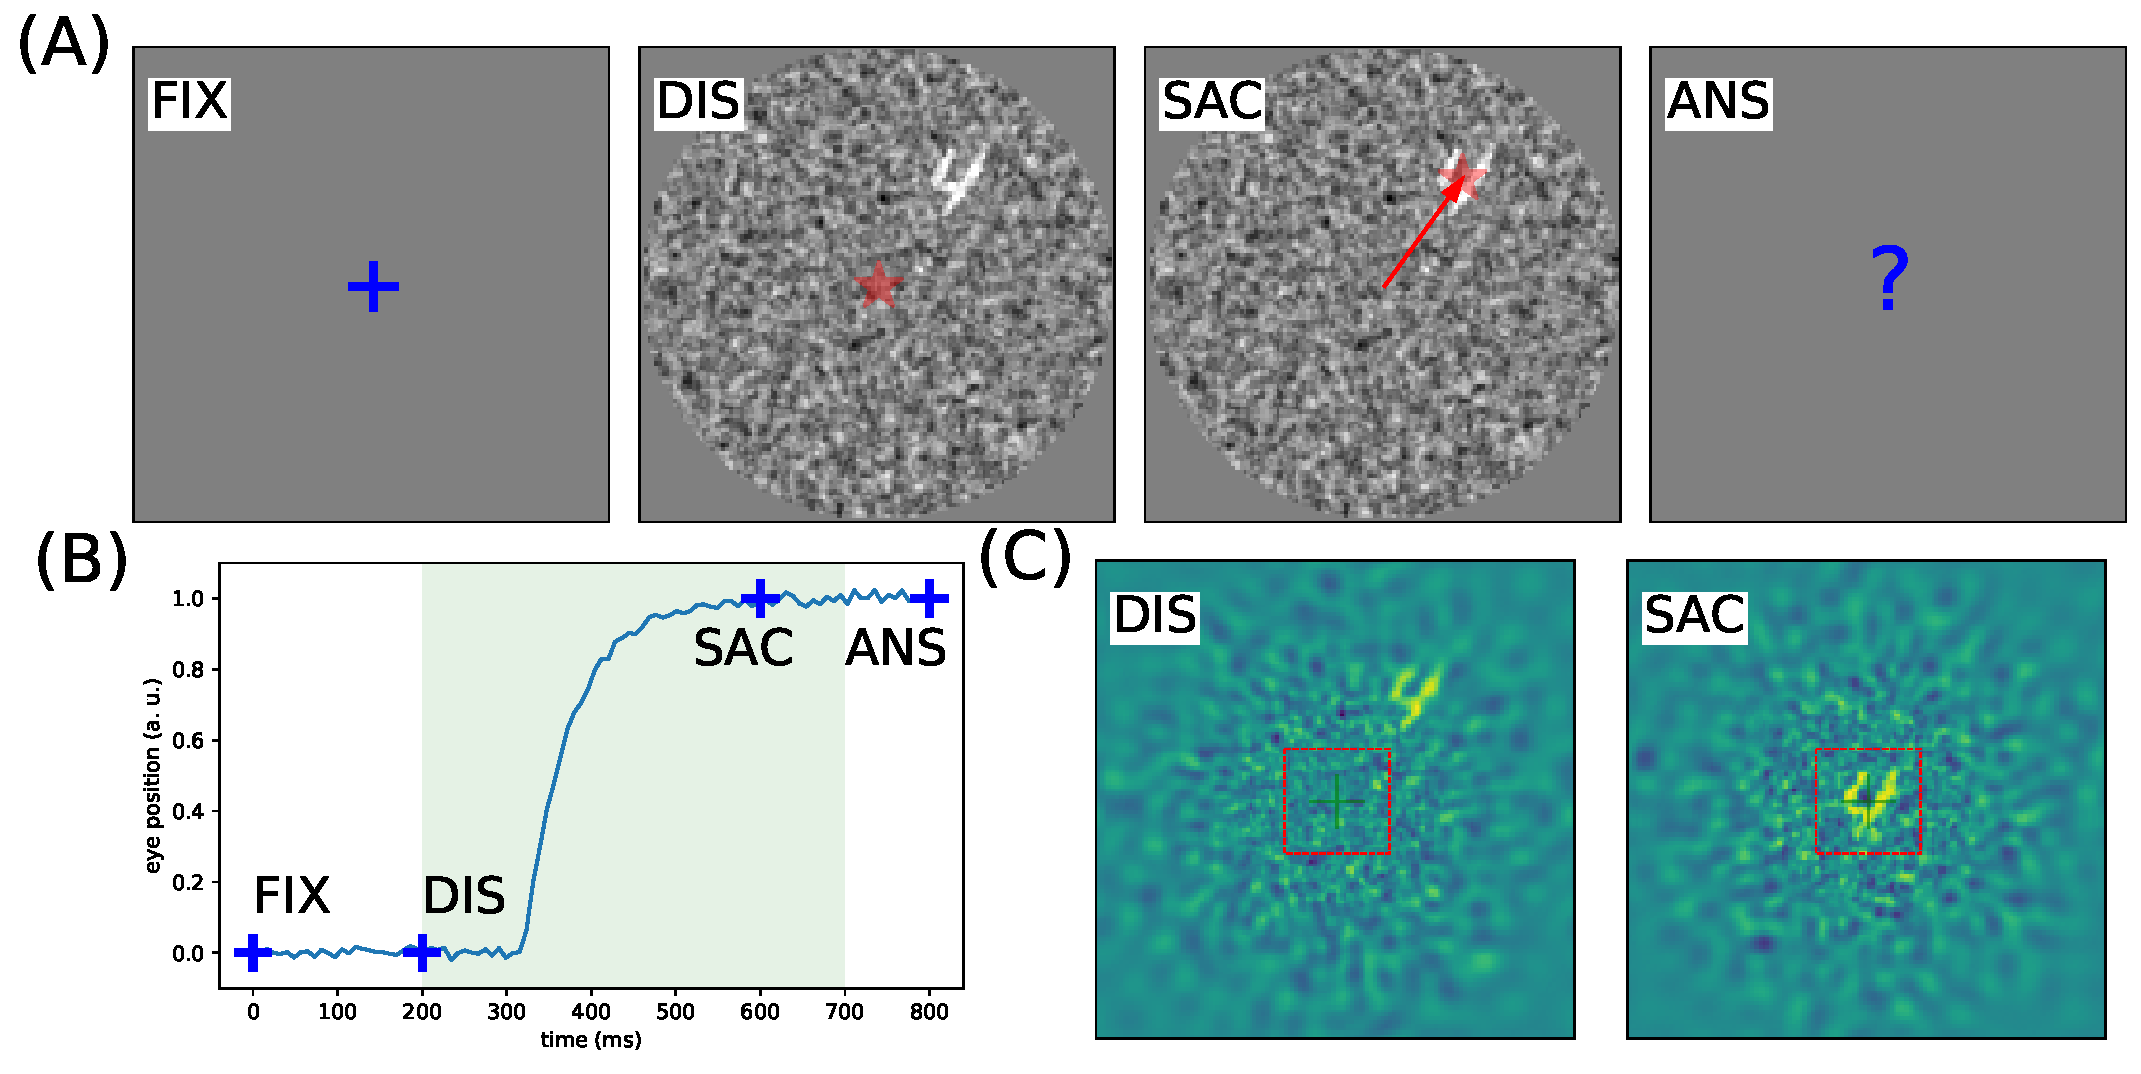
\includegraphics[width=\linewidth]{fig_intro}}%{fig_methods}}
\caption{
{\bf Methods for simulating active vision}:
\A We first define the model which generates images. It is composed of three different random processes: one choosing a sample image from the MNIST database (of size $28\times 28$) and placing it at a random position within the circular mask on the $128\times 128$ display. Then, this image is rectified and multiplied by a contrast factor and finally embedded in a natural-like noise with characterized by the noise contrast, mean spatial frequency and bandwidth~\citep{Sanz12}. %
\B The full-sized images are transformed into a retinal image which will be fed to the ``where'' pathway. This is implemented by a bank of filters whose centers are positioned on a log-polar grid and whose radius increases proportionally with eccentricity. In addition, a similar topographic map is used to represent the accuracy of each hypothetical position of a saccade, as represented by the collicular map. %
\C The ``where'' pathway is implemented by a three-layered neural network consisting of the retinal input, two hidden layers with $1000$ units each and a collicular output. Each unit is associated with a ReLU non-linearity. To learn to associate the output of the network with the ground truth, supervised training is performed using back-propagation with a binary cross entropy loss. This scalar measures the distance between both distributions (it is always positive and null if and only if they are equal). The network learns in about $20$ epochs as shown by the decrease of the loss function. Overlaid is the associated accuracy of the full active agent. This is computed by classifying the foveal image using the ``what'' pathway, after centering the gaze using the result of the ``where pathway''. This shows a gradual increase in accuracy from the baseline ($10\%$) to approximately an average of $X80.0X\%$. %
		\label{fig:methods}}%
\end{figure}%
%%------------------------------%
%
\subsection{Exteroceptive Generative model}
%=================================================================
It is first necessary to quantitatively define the generative model for input display images as shown first in Figure~\ref{fig:intro}-A (\DIS ) and as implemented in Figure~\ref{fig:methods}-A.

\paragraph{Targets.} Following a common hypothesis regarding active vision, visual scenes will consist of a single visual object of interest. We will use the MNIST database of handwritten digits introduced by~\citep{Lecun1998}. Indeed, we are here focused on the problem of localization (``where'' pathway) and classification solutions (``what'' pathway) abound for this class of targets. Samples are drawn from a database of $60000$ grayscale $28\times 28$ pixels images and separated between a training and a validation set (see below the description of the ``where'' network).
\paragraph{Full-scale images.} For each sample, we may now draw a random position in a full-scale image of $128\times 128$. To enforce isotropic saccades, we define a centered circular mask covering the image (of radius $64$ pixels) and the position is such that the embedded sample fits entirely into that circular mask.
\paragraph{Background noise setting. } To provide with a realistic background noise, we generated synthetic textures~\citep{Sanz12} using a third random process. These textured images are of the same size of the full-image. These static images are designed to fit well with the statistics of natural images. We chose an isotropic setting where textures are characterized by solely two parameters. One controls the median spatial frequency $sf_0$ of this noise, while the other controls the bandwidth around this central spatial frequency. Equivalently, these can be considered as the band-pass filtering of random white noise images. Finally, these images are rectified to have a normalized contrast.
\paragraph{Adding signal and noise. } Finally, both the noise and the target image are merged into a single image. We have used two different strategies. In a first strategy emulating a transparent association, we computed the average luminance at each pixel, while in a second strategy emulating an opaque association, we choose for each pixel the maximal value. The quantitative difference were tested in simulations, but proved to have a marginal importance.
%
\subsection{Interoceptive generative model}
%=================================================================
%
We will now define the simplified anatomy of our agent, which is composed of two separate pathways.



\paragraph{Foveal vision and the ``what'' pathway}
First, foveal vision is defined as the $28\times 28$ pixels image centered at the point of fixation (see dashed red box in Figure~\ref{fig:intro}-C). This image is then directly passed to the agent's visual categorical pathway (the ``What'' pathway). This is realized by the known ``LeNet'' classifier~\citep{Lecun1998}, that processes the $28 \times 28$ central pixels to identify the target category. Such a network is directly provided (and unmodified) by the pyTorch library~\citep{Paszke17}, and consists of a 3-layered Convolutional Neural Network. It is trained over the (centered) MNIST database after approx $20$ training epochs. Input images are rectified (with a mean and standard deviation of respectively $0.1307$ and $0.3081$). The network outputs a vector representing the probability of detecting each of the $10$ digits. We use the argument of the output neuron with maximum probability, to categorize each image. This strategy achieves an average $98.7\%$ accuracy on the validation dataset~\citep{Lecun1998}. %

\paragraph{Retinal transform: Peripheral vision and log Polar encoding}
First, both the visual features and the expected target position may to be expressed in retinal coordinates which we choose here to be log-polar as it provides a good fit with observations in mammals~\citep{Traver10}. On the visual side, we extracted local visual features as oriented edges  as the combination of the retinotopic transform with that of the primary visual cortex~\citep{Fischer2007a}. The centers of these first and second order orientation filters are radially organized around the center of fixation, with small and tightened receptive fields at the center and more large and scarce receptive fields at the periphery, see  Figure~\ref{fig:methods}-B. The size of the filters increases proportionally to eccentricity. The filters are organized in $10$ spatial eccentricity scales (respectively placed at around $2$, $3$, $4.5$, $6.5$, $9$, $13$, $18$, $26$, $36.5$ , and $51.3$ pixels from the center) and $16$ different azimuth angles allowing them to cover most of the original $128 \times 128 $ image. At each of these position, we computed $10$ different edge orientations and $2$ different phases (symmetric and anti-symmetric) using log-Gabor filters~\citep{Fischer2007a}. This finally implements a (fixed) bank of linear filters which model the receptive fields of the input to the primary visual cortex.

From any input image ($128\times 128=16384$ pixels) is linearly transformed into a retinal activity vector $\boldsymbol{x}$. Note that to ensure balace of the coefficients across scales, the images are first whitened. In practice, the length of this vector is $1600$ such that the retinal filter compresses the original image by about 90\%, with high spatial frequencies preserved at the center and only low spatial frequencies conserved at the periphery. In practice, this filters are pre-computed and placed into a matrix for a rapid transform of batches of input displays into retinal transforms. In practice this matrix transformation allows also the evaluation of a reconstructed visual image given a retinal activity vector thanks to the pseudo-inverse matrix of the forward transform matrix. In summary, the full-sized images are transformed into a peripheral retinal image which will be fed to the ``where'' pathway.

\paragraph{Collicular representation: accuracy map}
We will now define the output of the ``Where'' pathway as an \emph{accuracy map} representing the probability of the presence of a target in the visual field, independently of its identity. As the retinotopic map, this target accuracy map is also organized radially in a log-polar fashion, making the target position estimate more precise at the center and fuzzier at the periphery. This modeling choice is reminiscent of the approximate log-polar organization of the superior colliculus (SC) motor map. In ecological conditions, the accuracy map is trained by sampling, i.e. by "trial and error", using for instance corrective saccades to compute (a posteriori) the probability of a correct localization. In a computer simulation however, this induces a combinatorial explosion which does render the calculation not amenable.

However, as we generated the display, we know the position of the target (which is hidden to the agent). Moreover, we observed that we could also evaluate the accuracy of the classifier (that is the fixed ``what'' pathway) knowing the translational shift imposed to the input foveal image by a saccade of known amplitude. Knowing the size of the $28\times 28$ input image, this generates a $55\times 55$ accuracy map (larger shift correspond to a target outside the fovea and necessary an accuracy at the chance level of $10\%$). This classifier displays a high accuracy at the center (with a value of $98.7\%$ corresponding to the validation score without any translational shift), and a fast decreasing accuracy with target eccentricity, as shown in Figure~\ref{fig:results}-D. By assuming ergodicity, knowing this centered accuracy map, this allows us to rapidly predict for each visual display the full accuracy map at each pixel by shifting the centered accuracy map on the true position of the target. Such a computational shortcut is allowed by the independence of the categorical performance with position thanks to the independence which is implemented in the exteroceptive generative model.

Finally, we will project this full accuracy map on the collicular map to compute the accuracy of each hypothetical saccade in the collicular space (see  Figure~\ref{fig:methods}-B, "True"). In practice, we will use the energy of the filters at each position as a proxy to quantify the projection from the visual space of the display to the collicular space. This generates a filter bank at $10$ spatial eccentricity scales and $16$ different azimuth angles, and $160$ collicular receptive fields. Each filter is normalized such that the value at each collicular position is the average of the values which are integrated in visual space. Applied to the full sized ground truth accuracy map computed in display space, this gives an accuracy map at different location of motor space. Such collicular transform is again implemented by a simple matrix multiplication which can be pre-computed and particularly is rapid to compute. Practically, this also allows to compute an inverse transform using the pseudo-inverse matrix of the forward transform. In particular, we will use that inverse transform to represent the accuracy predicted by any given collicular vector, but also to compute the position in display space of maximal accuracy.

\subsection{Implementing the ``where'' pathway}
%=================================================================


\paragraph{Classifier training using deep learning}
Modern parametric classifiers are composed of many layers (hence the term ``Deep Learning'') that can be trained through gradient descent over arbitrary input and output feature spaces. The ease of use of those tightly optimized training algorithms allow to quantify the difficulty of a task through the failure or success of such training. Consider the retinal transform $\boldsymbol{x}$ as the input and a log-polar retinotopic vector $\boldsymbol{a}$ made of $n$ Bernouilli probabilities (success probabilities) as the output. Following the active inference framework, we will train the network to predict the distribution $\boldsymbol{a}$ knowing the retinal input $\boldsymbol{x}$ by comparing it to the known ground truth distribution computed over the collicular map. As a loss function, we will naturally use the Kullback-Leibler divergence between the ground truth and the predicted map.

%The ``What'' pathway will be given from the literature. In contrast, the ``Where'' pathway takes the into account in order to tell whether a target is present at the different peripheral locations, in order to monitor future saccades. 


In practice, the parametric neural network is made of an input (retinal) layer, two fully connected hidden layers of size $500$ and $2000$ units respectively and an output layer, with ReLu activation between each layer, except at the output which uses a sigmoid function to ensure that the output is compatible with the representation of a likelihood. In addition, we tested the effect of $50 \%$ drop-out on the last hidden layer. Another improvement in convergence speed was obtained by using Batch normalization. The network is trained over $500,000$ saccades on full-images, using the binary cross-entropy loss as the error signal, with a learning rate equal to $10^{-4}$ and stochastic gradient descent with a momentum to improve convergence. The training is done for $25$ epochs in about $1$ hours on a laptop. The code is written in Python with pyTorch library~\citep{Paszke17}. The full scripts for reproducing the figures and extending the results to a full range of parameters is available at \url{https://github.com/laurentperrinet/WhereIsMyMNIST}. % TODO: change to https://github.com/SpikeAI/DauceAlbigesPerrinet19 when public


% !TEX root = paper.tex
% !TEX encoding = UTF-8 Unicode
% -*- coding: UTF-8; -*-
% vim: set fenc=utf-8
% !TEX spellcheck = en-US
%=================================================================
\section{Results}
\label{sec:results}
%=================================================================
%=================================================================
\subsection{Inferring where to look}
%=================================================================
After training the network, we evaluated simulations of the final accuracy at the landing of the predicted saccade (see Figure~\ref{fig:results}). For each different visual display (a different digit at a different position), a retinocentric visual input is processed (figure \ref{fig:results}-A), providing a predicted accuracy map (figure \ref{fig:results}-B) that can be compared to the actual future accuracy. Then a saccade is carried out based on the most probable position as computed from the predicted accuracy map (figure \ref{fig:results}-C), and the final accuracy is computed from the ``what'' pathway using LeNet model. This is repeated $1,000$ times at different eccentricities, and the final average accuracy is shown as blue bars on figure \ref{fig:results}-D. It is compared to a central classifier trying to predict the category without doing a saccade (orange bars). As expected, the accuracy decreases with the eccentricity, for the targets become less and less visible in the periphery. The decrease is very rapid in the central classifier case: the accuracy drops to the baseline level %$50 \%$
after the third scale, which corresponds to a $4.6$ pixels radius around the center of fixation). In contrast, issuing a saccade is beneficial in up to $26$ pixels around the fixation center, allowing a much wider covering of the initial image. The difference between the two distributions forms an ``accuracy gain'', that quantifies the benefit of active inference with respect to a central prior, interpreted as the information gain provided by the ``Where'' pathway.
%------------------------------%fig_params
%: see Figure~\ref{fig:results}
\begin{figure}[t!]%%[p!]
%\flushleft{\bf (A) \hspace{4.2cm} (B) \hspace{2cm} (C) \hspace{4cm} (D)\hspace{6cm}}
\centering{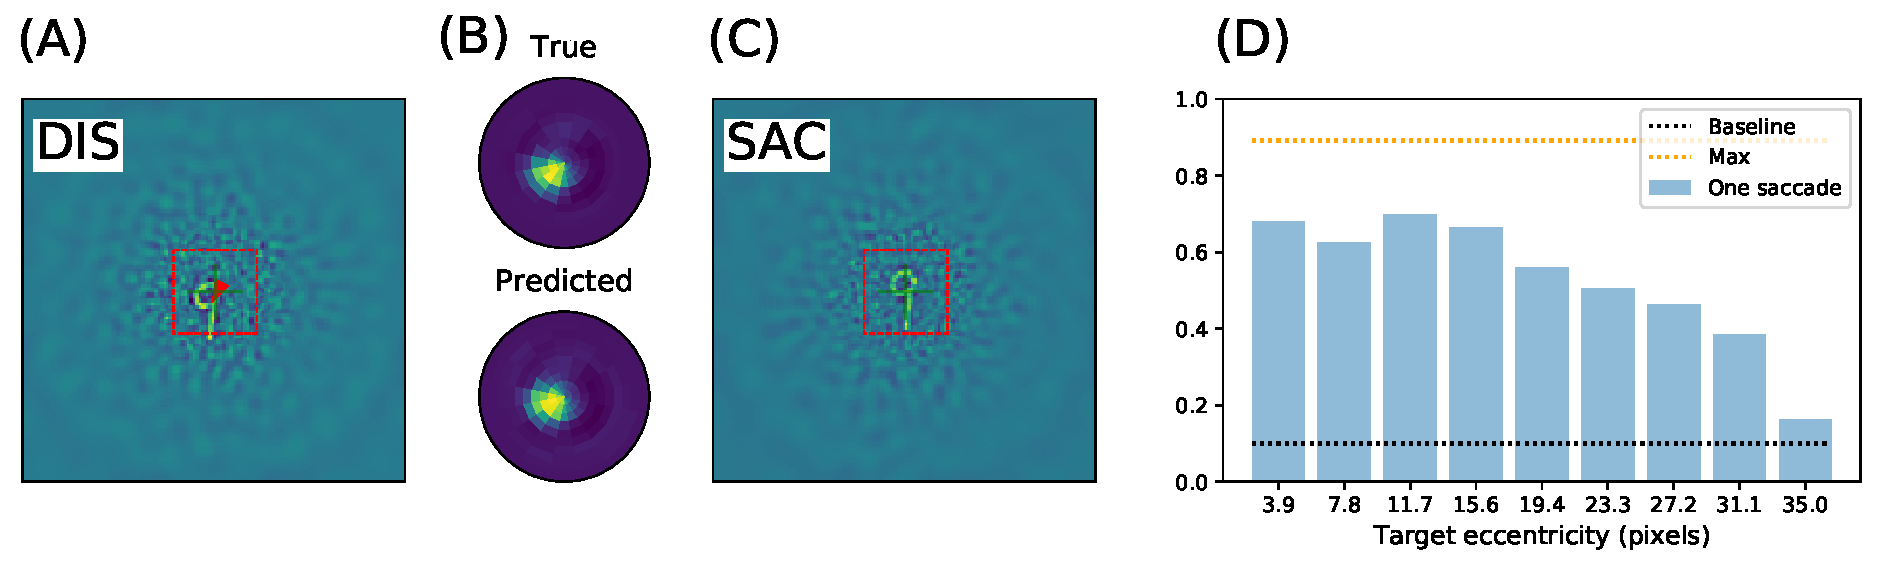
\includegraphics[width=\linewidth]{fig_result}}
\caption{
{\bf Simulated active vision agent}:
\A The visual display (\DIS , see also  Figure~\ref{fig:intro}-C)  is transformed into a retinotopic representation which is used as the input of a multi-layer neural network implementing the ``where'' pathway, that transforms the retinal image into an accuracy map. %
\B We show after training a typical network output  ('Predicted') as compared  with the ground truth ('True'). %
\C The network output allows to generate a saccade to the most likely target position in visual space and to recenter the retinotopic map (\SAC ), making possible to estimate a final classification rate. %
\D The active vision agent is tested at different eccentricities (in pixels). Orange bars: accuracy of a central classifier ('No saccade') with respect to the target's eccentricity, averaged over 1,000 trials per eccentricity scale. Blue bars: Final classification rate after one saccade predicted by the ``Where'' pathway.
\label{fig:results}}%
\end{figure}%
%%------------------------------%
% energy consumption

% inhibition of return
As our saccade selection algorithm may implement the essential operations done in the ``Where'' pathway, the central classifier may also reflect the response of the ``What'' pathway,
%A particular property of our agent is that at the time when the initial input is presented, two independent inferences are implemented. First, a
%The classification performed by the ``What'' pathway
giving the potential category of the digit. %Second, an accuracy map is predicted by the 'Where' pathway.
It is therefore possible to compare the two accuracy estimates to chose the most appropriate action: it may be that the  accuracy is best in the ``What'' pathway and in that case no saccade is produced.
The decision frontier lies between the first and the second spatial scale, allowing to pursue micro-saccades in the close vicinity of the target (2-3 pixels), in order to achieve a perfect centering.
In the other decision case, the ''What'' accuracy can still be considered to update the ``Where'' accuracy.
%Indeed, one knows in particular the accuracy of the 'what' pathway when imposing small shifts to the input.
This allows in particular to ``explain away" the current position of the fixation and the neighboring ones.
%(see line 'No saccade' in figure~\ref{fig:results}).
Such heuristic gives a principled formulation of the inhibition of return mechanism which is an important aspect for modeling saccades~\citep{Itti01}. In particular, we predict that such a mechanism is dependent on the class of inputs, and would be different for searching for faces as compared to digits.

\subsection{Quantitative role of parameters}
%=================================================================
%------------------------------%
%: see Figure~\ref{fig:params}
\begin{figure}[t!]%%[p!]
%\flushleft{\bf (A) \hspace{4.2cm} (B) \hspace{2cm} (C) \hspace{4cm} (D)\hspace{6cm}}
\centering{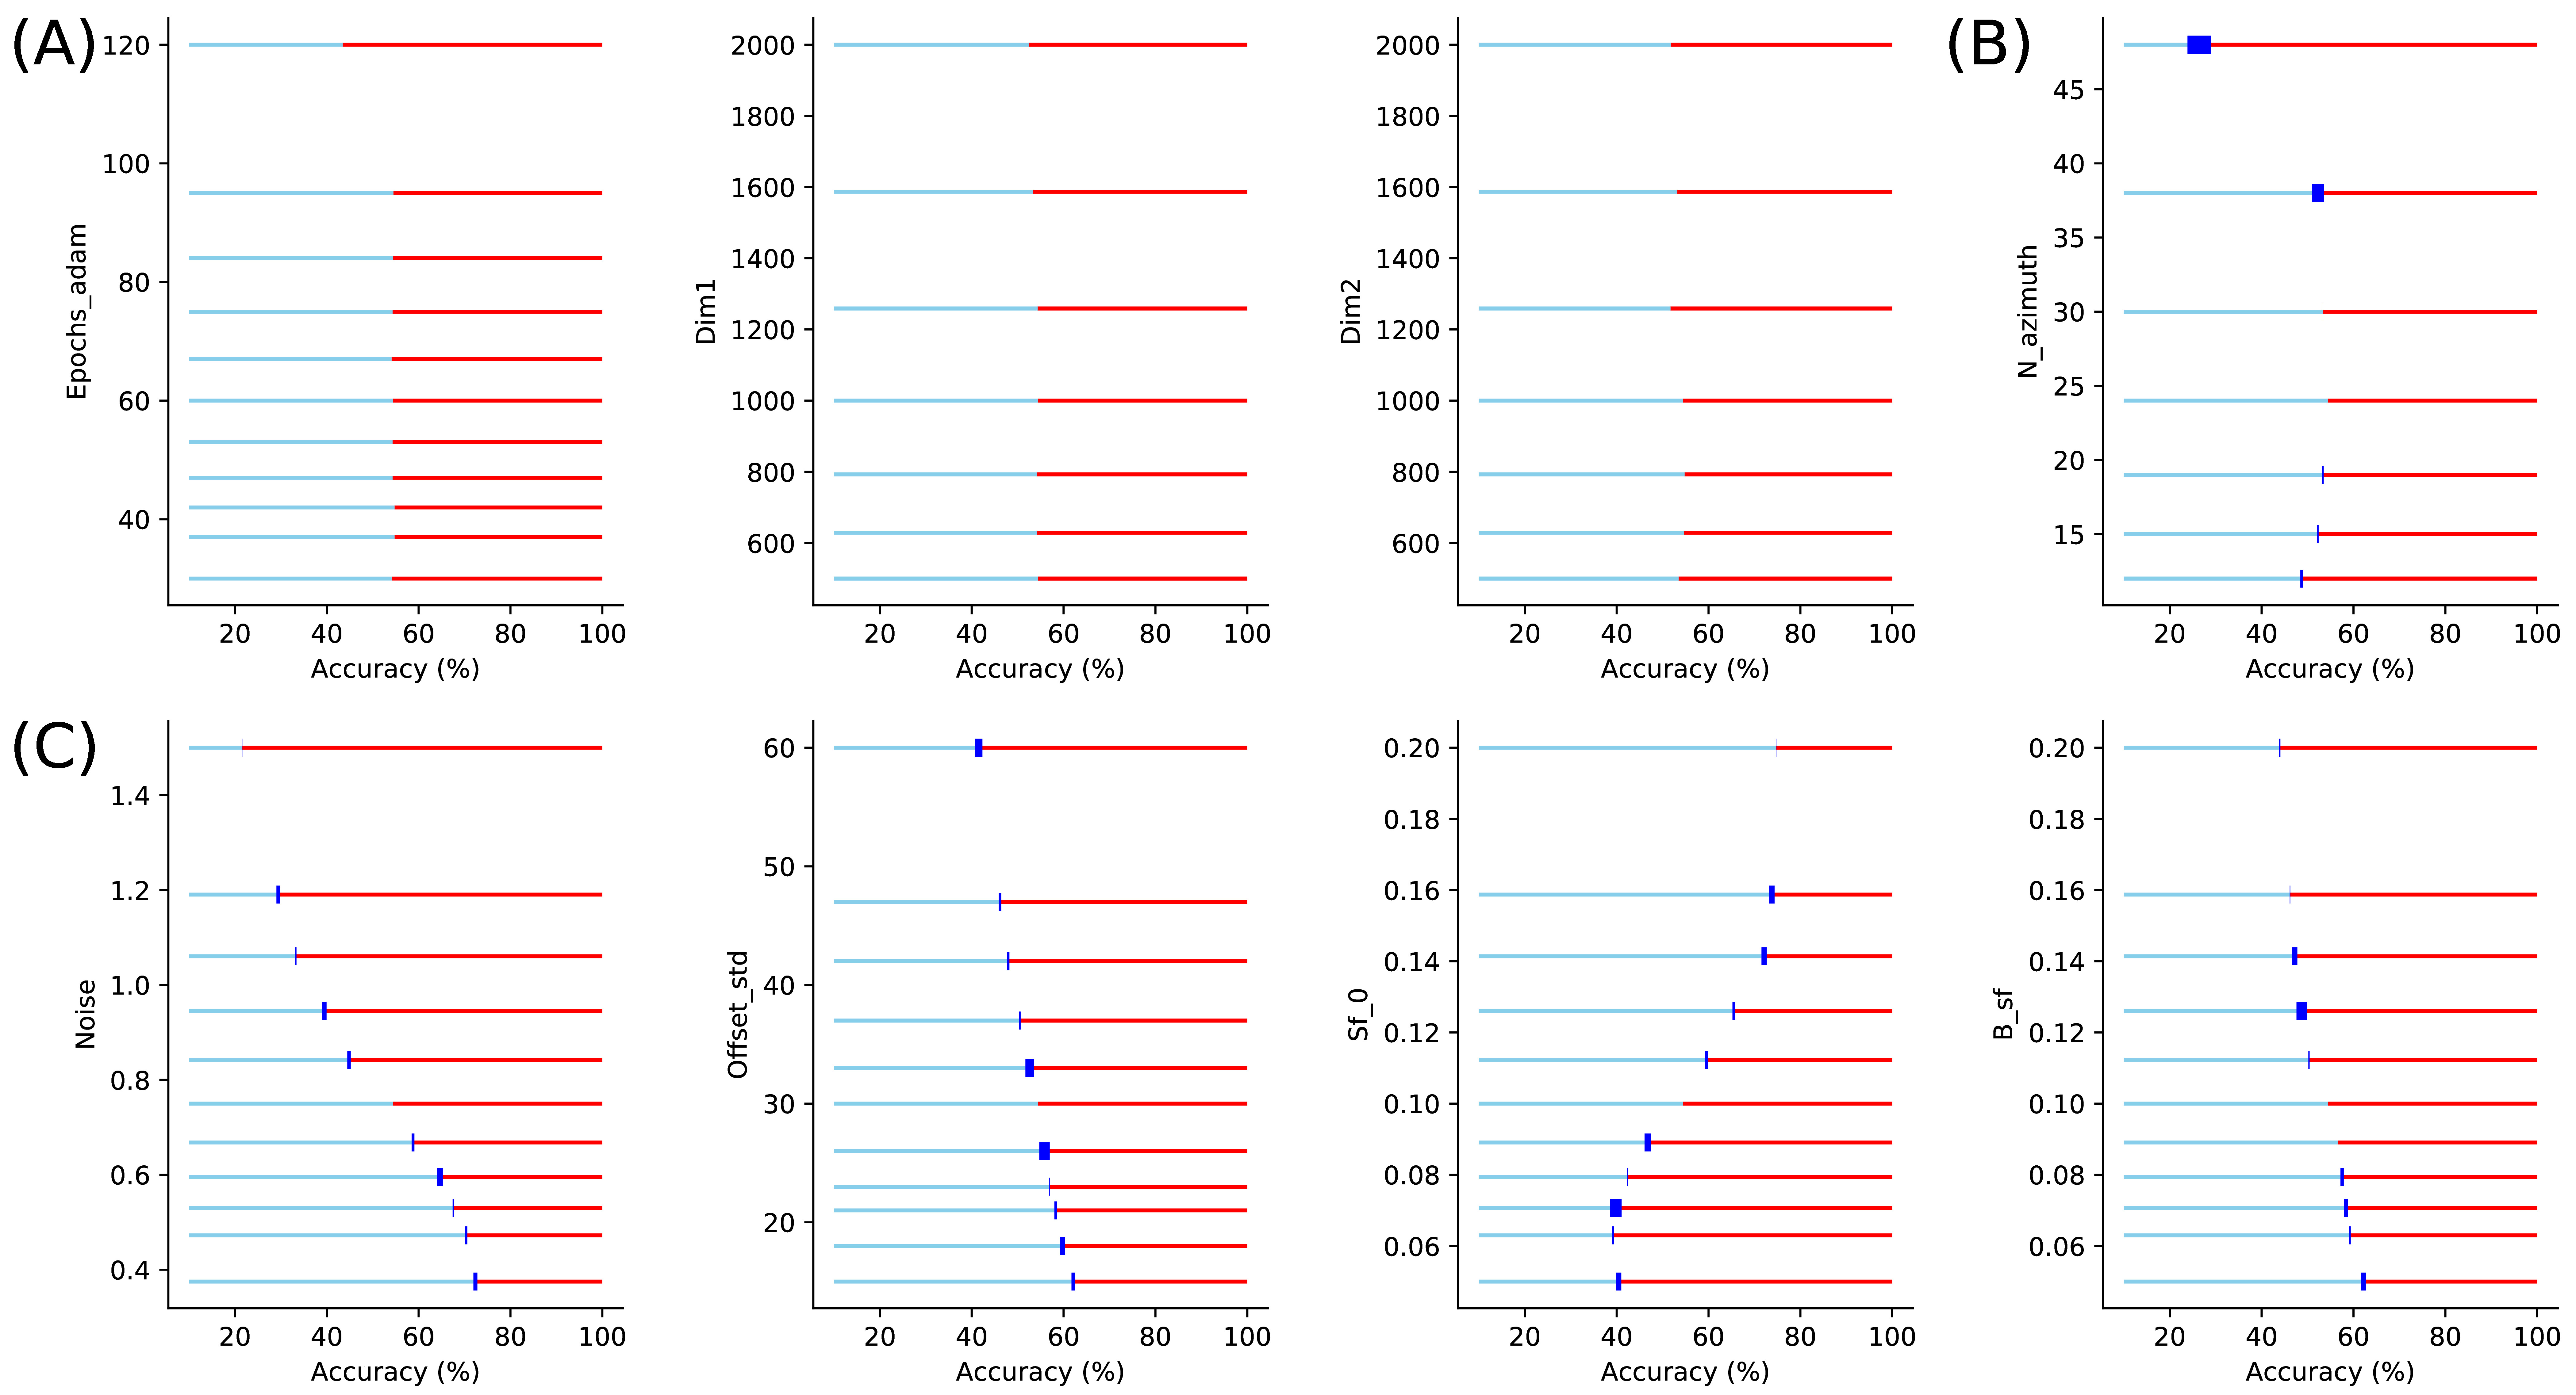
\includegraphics[width=\linewidth]{fig_params}}
\caption{
{\bf Quantitative role of parameters}:
\A The visual display (\DIS , see also  Figure~\ref{fig:intro}-C)  is transformed into a retinotopic representation which is used as the input of a multi-layer neural network implementing the ``where'' pathway, that transforms the retinal image into an accuracy map. %
\B We show after training a typical network output  ('Predicted') as compared  with the ground truth ('True'). %
\C The network output allows to generate a saccade to the most likely target position in visual space and to recenter the retinotopic map (\SAC ), making possible to estimate a final classification rate. %
\D The active vision agent is tested at different eccentricities (in pixels). Orange bars: accuracy of a central classifier ('No saccade') with respect to  function of the target eccentricity averaged over 1,000 trials per eccentricity scale. Blue bars: Final classification rate after one saccade predicted by the ``Where'' pathway.
\label{fig:params}}%
\end{figure}%
%%------------------------------%

\newpage

% !TEX root = DauceAlbigesPerrinet2020.tex
% !TEX encoding = UTF-8 Unicode
% -*- coding: UTF-8; -*-
% vim: set fenc=utf-8
% !TEX spellcheck = en-US
\section{Discussion} \label{sec:discussion}
\subsection{Summary}
%
In summary, we have proposed a visuomotor action-selection model that implements a focal accuracy-seeking policy across the image. Our main modeling assumption here is an \emph{accuracy-driven} monitoring of action, stating in short that the ventral classification accuracy drives the dorsal selection on an accuracy map. The comparison of both accuracies amounts either to select a saccade or to keep the eye focused at the center, so as to identify the target. The predicted accuracy map has, in our case, the role of a value-based action selection map, as it is the case in model-free reinforcement learning. However, it also owns a probabilistic interpretation, making it possible to combine concurrent accuracy predictions, such as the ones done through the ``What'' and the ``Where'' pathways. This allows in particulart to explain more elaborate aspects of the whole decision making processes, such as the inhibition of return~\cite{Itti01}, without further specific heuristic.

Moreover, one crucial aspect highlighted by our model is the importance of centering objects in recognition. Despite the robust translation invariance observed on the ``What'' pathway, a small tolerance radius of about $4$ pixels around the target's center needs to be respected to maximize the classification accuracy. The translation invariance is in our case an effect of the max-pooling operations in the convolutional layers, build-in at the core of the ``What'' layer. This relates to the idea of finding an absolute referential for an object, for which the recognition is easier. If the center of fixation is fixed, the log-polar encoding of an object has the notable properties to map object rotations and scalings toward translations in the radial and angular directions of the visual domain~\cite{Traver10}. Extensions to scale and rotation invariance would in principle be feasible through central log polar encoding, with little additional computational cost. This prospect is left for future work.
%
\subsection{Comparison with other models}
%%
A lot of computer models found in the literature reflect to some degree the foveal/sequential visual processing principles developed here. Since the question of a normative and quantitative comparison with them is important, no specific or unified dataset is proposed at present to address this specific case. Every model found uses a different retinal encoding, different computing methodologies and different training datasets. We thus provide here a qualitative comparison with the more prominent computer-based focal vision models proposed in the literature.

First, active vision is of course an important topic in mainstream computer vision. In the case of image classification, it is considered as a way to improve object recognition by progressively increasing the definition over identified regions of interest, referred as ``recurrent attention''~\cite{mnih2014recurrent,fu2017look}. Standing on a similar mathematical background, recurrent attention is however at odd with the functioning of biological systems, with a mere distant analogy with the retinal principles of foveal-surround visual definition.

Phenomenological models, such as the one proposed in Najemnik and Geisler's seminal paper~\cite{Najemnik05}, rely on a rough simplification, with foveal center-surround acuity modeled as a response curve. Despite providing a bio-realistic account of sequential visual search, the model owns no foveal image processing implementation. Stemming on Najemnik and Geisler's principles, a trainable center-surround processing system was proposed in~\cite{Butko2010infomax}, with a sequential scan of an image in a face-detection task. However, the visual search task relies there on a systematic scan over a dynamically-blurred image, with all the visual processing delegated to standard feature detectors.

In contrast, the Akbas and Eckstein model (“foveated object detector”~\cite{akbas2017object}) uses an explicit bio-inspired log-polar encoding
for the peripheral processing, with trainable local features.
With a focus put on the processing effectiveness provided by this specific compression,
the model approaches the performance of state-of-the-art linear feature detectors, with multi-scale template matching (bounding box approach). However the use of
a local/linear template matching processing makes here again the analogy with the brain quite shallow.

Denil et al's paper~\cite{denil2012learning} is probably the one that shows the closest correspondence with our setup. It owns an identity pathway and a control pathway, in a What/Where fashion, just as ours. Interestingly, only the ``What'' pathway is neurally implemented using a random foveal/multi-fixation scan within the fixation zone. The ``Where'' pathway, in contrast, mainly implements object tracking, using particle filtering with a separately learned generative process. The direction of gaze is here chosen so as to minimize the target's position, speed and scale uncertainty, using the variance of the future beliefs as an uncertainty metric. The control part is thus much similar to a dynamic ROI tracking algorithm, with no direct correspondence with foveal visual search, or with the capability to recognize the target
%
\subsection{Perspectives}
%
We have thus provided here for the first time with a proof of concept that a log-polar retinotopy can efficiently serve object detection and identification over wide visual displays. Despite its simplicity, the generative model used to generate our visual display allowed to assess the effectiveness and robustness of our learning scheme, that should be extended in the future to more complex displays and more realistic closed-loop setups. In particular, the restricted $28\times28$ input used for the foveal processing is a mere placeholder, that should be replaced by more elaborate computer vision frameworks, such as Inception~\cite{szegedy2015going} or VGG-19~\cite{simonyan2014very}, that can handle a more ecological natural image classification.

The main advantage of our peripheral image processing is its cost-efficacy. Our full log-polar processing pathway consistently conserves the high compression rate performed by retina and V1 encoding up to the action selection level. The organization of both the visual filters and the action maps in concentric log-polar elements, with radially exponentially growing spatial covering, can thus serve as a baseline for a future sub-linear (logarithmic) complexity for visual search in computer vision. Our work thus illustrates one of the main advantages of using a focal/sequential visual processing framework, that is providing a way to process large images with a sub-linear processing cost. This may allow to detect an object in large visual environments, which should be particularly beneficial when the computing resources are under constraint, such as for drones or mobile robots.

If the methodology and principles developed here are clearly intended to deal with real images, an important contribution of the paper is providing principles that justify the separation between a ventral and a dorsal stream in the early visual pathways. If some forms of ``dual pathway models'' have been proposed in the past (through separating the central and the peripheral processing, like in~\cite{denil2012learning}, and also in one instance of the~\cite{akbas2017object} model), their guiding principles stem on computing efficacy rather than biological fidelity. We thus think that our principled ventral/dorsal concurrent processing, rooted on dorsal accuracy map predictions, is both important and novel.

Finally, our approach relies on a strong idealization, assuming the presence of a unique target. This is well adapted to a fast changing visual scene as is demonstrated by our ability to perform as fast as 5 saccades per second to detect faces in a cluttered environment~\cite{Martin18}. However, some visual scenes ---such as when looking at a painting in a museum--- allow for a longer inspection of its details. The presence of many targets in a scene should be addressed, which amounts to sequentially select targets, in combination with implementing a more elaborate inhibition of return mechanism to account for the trace of the performed saccades. This would generate more realistic visual scan-paths over images. Actual visual scan-paths over images could also be used to provide priors over action selection maps that should improve realism. Identified regions of interest may then be compared with the baseline bottom-up approaches, such as the low-level feature-based saliency maps~\cite{Itti01}. Maximizing the Information Gain over multiple targets needs to be envisioned with a more refined probabilistic framework extending previous models~\cite{Friston12}, which would include phenomena such as mutual exclusion over overt and covert targets. How the brain may combine and integrate these various probabilities is still an open question, that amounts to the fundamental binding problem. 

\newpage
\section*{General case: Visual information gain maximization}\label{sec:case1}

Consider a view $\boldsymbol{x}$ generated from a target $\boldsymbol{y}$ viewed at retinocentric position $\boldsymbol{u}$. 

Consider first that :
\begin{itemize}
	\item The generative model  $p(X|\boldsymbol{y}, \boldsymbol{u})$ is known
	\item The retinocentric position  $\boldsymbol{u}$ is known.
	\item The view $\boldsymbol{x}$ is known.
	\item The target category  $\boldsymbol{y}$ is unknown.
\end{itemize} 



The question comes how to choose the new retinocentric position $\boldsymbol{u}'$ in order to maximize the \emph{mutual information} between $\boldsymbol{x}|\boldsymbol{u}$ (current view) and $\boldsymbol{x}'|\boldsymbol{u}'$ (future view).

In general, the visual Information Gain between two visual fields $\boldsymbol{x}|\boldsymbol{u}$  and $\boldsymbol{x}'|\boldsymbol{u}'$ is:

\begin{align*}
\text{IG}(\boldsymbol{x}|\boldsymbol{u}; \boldsymbol{x}'| \boldsymbol{u}') 
&= -\log p(\boldsymbol{x}|\boldsymbol{u}) 
+ \log p(\boldsymbol{x}|\boldsymbol{u}, \boldsymbol{x}', \boldsymbol{u}')
\end{align*}

\paragraph{Information Gain Lower Bound}
Consider now that given  $\boldsymbol{x}$ and $\boldsymbol{u}$, the target category  $\boldsymbol{y}$ can be \emph{inferred} using Bayes rule, i.e.:
$$ P(Y|\boldsymbol{x}, \boldsymbol{u}) \propto  P(\boldsymbol{x}|Y, \boldsymbol{u}) $$
Then, it can be shown (see \cite{dauce2018}) that :
$$\text{IG}(\boldsymbol{x}|\boldsymbol{u}; \boldsymbol{x}'| \boldsymbol{u}') \geq \mathbb{E}_{\boldsymbol{y}\sim p(Y|\boldsymbol{x}, \boldsymbol{u})} \left[\log p(\boldsymbol{y}|\boldsymbol{x}', \boldsymbol{u}') - \log(\pi(\boldsymbol{y})) \right]$$
with  $\pi(\boldsymbol{y})$ the prior over the $\boldsymbol{y}$'s .
When the prior is uniform, the information gain lower bound (IGLB) simplifies to $\mathbb{E}_{\boldsymbol{y}\sim p(Y|\boldsymbol{x}, \boldsymbol{u})} \left[\log p(\boldsymbol{y}|\boldsymbol{x}', \boldsymbol{u}')\right] + c$, with $c$ a constant.

\paragraph{Predictive approach}
One can adopt a \emph{predictive} approach to choose the new eye orientation $\boldsymbol{e}'$:
\begin{itemize}
	\item First choose a new retinocentric position $\boldsymbol{u}'$ that will maximize the  information gain.
	\item Then choose $\boldsymbol{e}'$ such that $$\boldsymbol{z} - \boldsymbol{e}' = \boldsymbol{u}'$$ i.e. $$\boldsymbol{e}' = \boldsymbol{e} + \boldsymbol{u} - \boldsymbol{u}'$$
\end{itemize}

The predictive approach needs three predictive steps:
\begin{itemize}
	\item $p(Y|\boldsymbol{x}, \boldsymbol{u})$ is the current posterior over the target category inferred from the current observation,
	\item $\boldsymbol{x}'\sim p(X|\boldsymbol{y},\boldsymbol{u}')$ is the predicted view generated by the model assuming that the target $\boldsymbol{y}$ is seen from from $\boldsymbol{u}'$,
	\item and $p(\boldsymbol{y}|\boldsymbol{x}', \boldsymbol{u}')$ is the predicted posterior for   assumption $\boldsymbol{y}$, given $\boldsymbol{x}'$ and $\boldsymbol{u}'$.
\end{itemize}

Then the optimal new retinocentric position is:
\begin{align*}
\hat{\boldsymbol{u}}' &= \underset{\boldsymbol{u}' }{\text{ argmax }} 
 \mathbb{E}_{\boldsymbol{y}\sim p(Y|\boldsymbol{x}, \boldsymbol{u})}  
 \left[\mathbb{E}_{ \boldsymbol{x}' \sim p(X|\boldsymbol{y}, \boldsymbol{u}')}
 \left[\log p(\boldsymbol{y}|\boldsymbol{x}', \boldsymbol{u}')\right]\right]\\
  %&= \underset{\boldsymbol{u}' \in \mathcal{U}}{\text{ argmax }} A(\boldsymbol{u}'|\boldsymbol{x}, \boldsymbol{u})
\end{align*}

Taking $\delta \boldsymbol{e} = \boldsymbol{u} - \boldsymbol{u}'$, the optimal eye displacement is: 
\begin{align*}
\widehat{\delta\boldsymbol{e}} &= \underset{\delta\boldsymbol{e} }{\text{ argmax }} 
\mathbb{E}_{\boldsymbol{y}\sim p(Y|\boldsymbol{x}, \boldsymbol{u})}  
\left[\mathbb{E}_{ \boldsymbol{x}' \sim p(X|\boldsymbol{y}, \boldsymbol{u}- \delta \boldsymbol{e})}
\left[\log p(\boldsymbol{y}|\boldsymbol{x}', \boldsymbol{u}-\delta\boldsymbol{e})\right]\right]\\
%&= \underset{\delta\boldsymbol{e}}{\text{ argmax }} A(\delta\boldsymbol{e}|\boldsymbol{x}, \boldsymbol{u})
\end{align*}

%For each possible target identity $\boldsymbol{y}$, $A_{\boldsymbol{y}}(\boldsymbol{u}') = \mathbb{E}_{ \boldsymbol{x}' \sim p(X|\boldsymbol{y}, \boldsymbol{u}')}
%\left[\log p(\boldsymbol{y}|\boldsymbol{x}', \boldsymbol{u}')\right]$ is the \emph{class-specific log posterior} map and 




%Then:
%$$\tilde{A}_{\boldsymbol{y}}(\boldsymbol{u}') = \mathbb{E}_{ \boldsymbol{x}' \sim p(X|\boldsymbol{y}, \boldsymbol{u}')}$$

\emph{(TODO : Attention il faudrait à partir de maintenant une carte qui moyenne les log posteriors car l'espérance du log n'est pas  égale au log de l'espérance, i.e. $r_{\theta}^{\text{log}}(\boldsymbol{u}|q) = \mathbb{E}_{\boldsymbol{y}\sim q(Y)} \left[\mathbb{E}_{ \boldsymbol{x} \sim p(X|\boldsymbol{y}, \boldsymbol{u})}  \log p_\theta(\boldsymbol{y}|\boldsymbol{x}, \boldsymbol{u}) \right]$).}
\newline

\end{document}